\documentclass{standalone}
\usepackage{tikz}
\usetikzlibrary{patterns, positioning}
\usepackage[sfdefault]{ClearSans} %% option 'sfdefault' activates Clear Sans as the default text font
\usepackage[T1]{fontenc}

\begin{document}
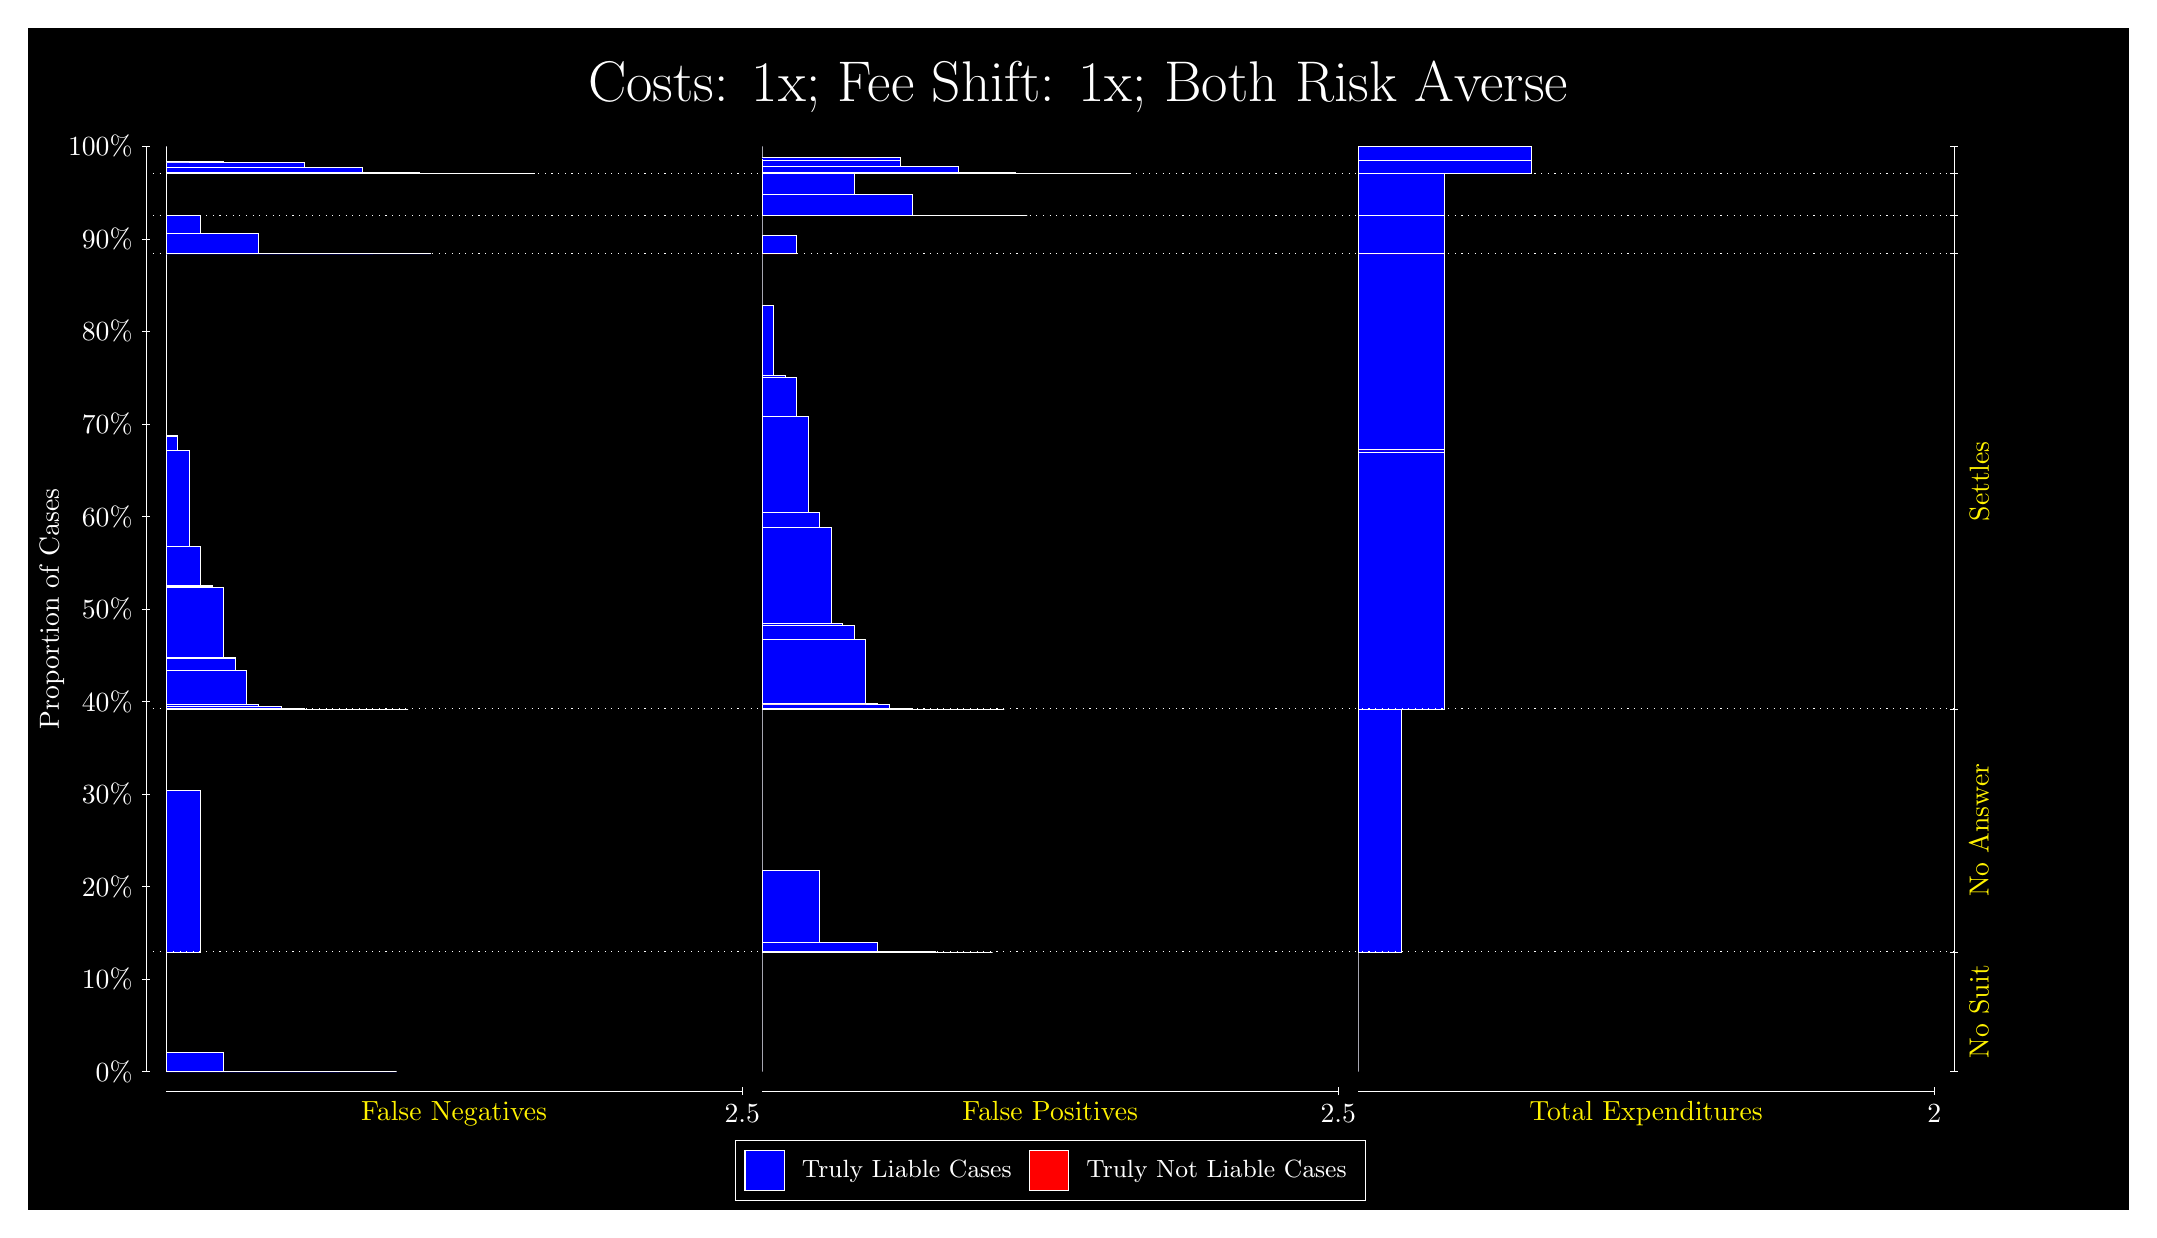
\begin{tikzpicture}
\draw[fill=black] (0,0) rectangle (26.667,15);
\draw[text=white] (0,13.5) rectangle (26.667,15) node[midway] {\huge Costs: 1x; Fee Shift: 1x; Both Risk Averse};
\draw[white, very thin] (1.5,1.75) -- (1.5,13.5);
\node[rotate=90, text=white, anchor=center] at (0.3, 7.625) {Proportion of Cases};
\draw[white, very thin] (1.45,1.75) -- (1.55,1.75);
\node[text=white, anchor=east] at (1.45, 1.75) {0\%};
\draw[white, very thin] (1.45,2.925) -- (1.55,2.925);
\node[text=white, anchor=east] at (1.45, 2.925) {10\%};
\draw[white, very thin] (1.45,4.1) -- (1.55,4.1);
\node[text=white, anchor=east] at (1.45, 4.1) {20\%};
\draw[white, very thin] (1.45,5.275) -- (1.55,5.275);
\node[text=white, anchor=east] at (1.45, 5.275) {30\%};
\draw[white, very thin] (1.45,6.45) -- (1.55,6.45);
\node[text=white, anchor=east] at (1.45, 6.45) {40\%};
\draw[white, very thin] (1.45,7.625) -- (1.55,7.625);
\node[text=white, anchor=east] at (1.45, 7.625) {50\%};
\draw[white, very thin] (1.45,8.8) -- (1.55,8.8);
\node[text=white, anchor=east] at (1.45, 8.8) {60\%};
\draw[white, very thin] (1.45,9.975) -- (1.55,9.975);
\node[text=white, anchor=east] at (1.45, 9.975) {70\%};
\draw[white, very thin] (1.45,11.15) -- (1.55,11.15);
\node[text=white, anchor=east] at (1.45, 11.15) {80\%};
\draw[white, very thin] (1.45,12.325) -- (1.55,12.325);
\node[text=white, anchor=east] at (1.45, 12.325) {90\%};
\draw[white, very thin] (1.45,13.5) -- (1.55,13.5);
\node[text=white, anchor=east] at (1.45, 13.5) {100\%};

\draw[white, very thin] (24.457,1.75) -- (24.457,13.5);
\draw[white, very thin] (24.407,1.75) -- (24.507,1.75);
\node[anchor=west] at (24.407, 1.75) {};
\draw[white, very thin] (24.407,3.2701) -- (24.507,3.2701);
\node[anchor=west] at (24.407, 3.2701) {};
\draw[white, very thin] (24.407,6.3562) -- (24.507,6.3562);
\node[anchor=west] at (24.407, 6.3562) {};
\draw[white, very thin] (24.407,12.138) -- (24.507,12.138);
\node[anchor=west] at (24.407, 12.138) {};
\draw[white, very thin] (24.407,12.622) -- (24.507,12.622);
\node[anchor=west] at (24.407, 12.622) {};
\draw[white, very thin] (24.407,13.16) -- (24.507,13.16);
\node[anchor=west] at (24.407, 13.16) {};
\draw[white, very thin] (24.407,13.5) -- (24.507,13.5);
\node[anchor=west] at (24.407, 13.5) {};

\draw[white, very thin, fill=blue] (1.75,1.75) rectangle (4.6775,1.75);
\draw[white, very thin, fill=blue] (1.75,1.75) rectangle (3.9457,1.75);
\draw[white, very thin, fill=blue] (1.75,1.75) rectangle (3.2138,1.7521);
\draw[white, very thin, fill=blue] (1.75,1.7521) rectangle (2.4819,1.9989);
\draw[white, very thin, fill=red] (1.75,1.9989) rectangle (1.75,1.9989);
\draw[white, very thin, fill=blue] (1.75,1.9989) rectangle (1.75,3.2701);
\draw[white, very thin, fill=blue] (1.75,3.2701) rectangle (2.1891,5.3234);
\draw[white, very thin, fill=red] (1.75,5.3234) rectangle (1.75,5.3234);
\draw[white, very thin, fill=blue] (1.75,5.3234) rectangle (1.75,6.3562);
\draw[white, very thin, fill=blue] (1.75,6.3562) rectangle (4.8239,6.3562);
\draw[white, very thin, fill=blue] (1.75,6.3562) rectangle (4.5312,6.3562);
\draw[white, very thin, fill=blue] (1.75,6.3562) rectangle (4.2384,6.3562);
\draw[white, very thin, fill=blue] (1.75,6.3562) rectangle (4.092,6.3562);
\draw[white, very thin, fill=blue] (1.75,6.3562) rectangle (3.9457,6.3562);
\draw[white, very thin, fill=blue] (1.75,6.3562) rectangle (3.7993,6.3562);
\draw[white, very thin, fill=blue] (1.75,6.3562) rectangle (3.6529,6.3562);
\draw[white, very thin, fill=blue] (1.75,6.3562) rectangle (3.5065,6.3667);
\draw[white, very thin, fill=blue] (1.75,6.3667) rectangle (3.3602,6.3676);
\draw[white, very thin, fill=blue] (1.75,6.3676) rectangle (3.2138,6.3907);
\draw[white, very thin, fill=blue] (1.75,6.3907) rectangle (3.0674,6.3908);
\draw[white, very thin, fill=blue] (1.75,6.3908) rectangle (3.0674,6.3912);
\draw[white, very thin, fill=blue] (1.75,6.3912) rectangle (2.921,6.4129);
\draw[white, very thin, fill=blue] (1.75,6.4129) rectangle (2.7746,6.8502);
\draw[white, very thin, fill=blue] (1.75,6.8502) rectangle (2.6283,6.9945);
\draw[white, very thin, fill=blue] (1.75,6.9945) rectangle (2.6283,7.012);
\draw[white, very thin, fill=blue] (1.75,7.012) rectangle (2.4819,7.9);
\draw[white, very thin, fill=blue] (1.75,7.9) rectangle (2.3355,7.9188);
\draw[white, very thin, fill=blue] (1.75,7.9188) rectangle (2.3355,7.9264);
\draw[white, very thin, fill=blue] (1.75,7.9264) rectangle (2.1891,8.4178);
\draw[white, very thin, fill=blue] (1.75,8.4178) rectangle (2.0428,9.6371);
\draw[white, very thin, fill=blue] (1.75,9.6371) rectangle (1.8964,9.8186);
\draw[white, very thin, fill=blue] (1.75,9.8186) rectangle (1.8964,9.8325);
\draw[white, very thin, fill=red] (1.75,9.8325) rectangle (1.75,9.8325);
\draw[white, very thin, fill=blue] (1.75,9.8325) rectangle (1.75,12.138);
\draw[white, very thin, fill=blue] (1.75,12.138) rectangle (5.1167,12.138);
\draw[white, very thin, fill=blue] (1.75,12.138) rectangle (4.3848,12.138);
\draw[white, very thin, fill=blue] (1.75,12.138) rectangle (3.6529,12.143);
\draw[white, very thin, fill=blue] (1.75,12.143) rectangle (2.921,12.391);
\draw[white, very thin, fill=blue] (1.75,12.391) rectangle (2.1891,12.622);
\draw[white, very thin, fill=red] (1.75,12.622) rectangle (1.75,12.622);
\draw[white, very thin, fill=blue] (1.75,12.622) rectangle (2.1891,12.625);
\draw[white, very thin, fill=red] (1.75,12.625) rectangle (1.75,12.625);
\draw[white, very thin, fill=blue] (1.75,12.625) rectangle (1.75,13.16);
\draw[white, very thin, fill=blue] (1.75,13.16) rectangle (6.4341,13.16);
\draw[white, very thin, fill=blue] (1.75,13.16) rectangle (5.7022,13.16);
\draw[white, very thin, fill=blue] (1.75,13.16) rectangle (4.9703,13.165);
\draw[white, very thin, fill=blue] (1.75,13.165) rectangle (4.2384,13.238);
\draw[white, very thin, fill=blue] (1.75,13.238) rectangle (3.9457,13.238);
\draw[white, very thin, fill=blue] (1.75,13.238) rectangle (3.5065,13.298);
\draw[white, very thin, fill=blue] (1.75,13.298) rectangle (3.2138,13.298);
\draw[white, very thin, fill=blue] (1.75,13.298) rectangle (2.7746,13.299);
\draw[white, very thin, fill=blue] (1.75,13.299) rectangle (2.4819,13.304);
\draw[white, very thin, fill=blue] (1.75,13.304) rectangle (2.0428,13.304);
\draw[white, very thin, fill=red] (1.75,13.304) rectangle (1.75,13.304);
\draw[white, very thin, fill=blue] (1.75,13.304) rectangle (1.75,13.5);
\draw[white, very thin, fill=red] (9.3189,1.75) rectangle (9.3189,1.75);
\draw[white, very thin, fill=blue] (9.3189,1.75) rectangle (9.3189,3.2701);
\draw[white, very thin, fill=red] (9.3189,3.2701) rectangle (12.246,3.2701);
\draw[white, very thin, fill=blue] (9.3189,3.2701) rectangle (12.246,3.2701);
\draw[white, very thin, fill=blue] (9.3189,3.2701) rectangle (11.515,3.271);
\draw[white, very thin, fill=blue] (9.3189,3.271) rectangle (10.783,3.3973);
\draw[white, very thin, fill=blue] (9.3189,3.3973) rectangle (10.051,4.3029);
\draw[white, very thin, fill=blue] (9.3189,4.3029) rectangle (9.3189,6.3562);
\draw[white, very thin, fill=red] (9.3189,6.3562) rectangle (12.393,6.3562);
\draw[white, very thin, fill=blue] (9.3189,6.3562) rectangle (12.393,6.3562);
\draw[white, very thin, fill=red] (9.3189,6.3562) rectangle (11.807,6.3562);
\draw[white, very thin, fill=blue] (9.3189,6.3562) rectangle (11.807,6.3562);
\draw[white, very thin, fill=blue] (9.3189,6.3562) rectangle (11.661,6.3562);
\draw[white, very thin, fill=red] (9.3189,6.3562) rectangle (11.515,6.3562);
\draw[white, very thin, fill=blue] (9.3189,6.3562) rectangle (11.515,6.3562);
\draw[white, very thin, fill=red] (9.3189,6.3562) rectangle (11.222,6.3562);
\draw[white, very thin, fill=blue] (9.3189,6.3562) rectangle (11.222,6.3626);
\draw[white, very thin, fill=blue] (9.3189,6.3626) rectangle (11.075,6.3627);
\draw[white, very thin, fill=red] (9.3189,6.3627) rectangle (10.929,6.3627);
\draw[white, very thin, fill=blue] (9.3189,6.3627) rectangle (10.929,6.4186);
\draw[white, very thin, fill=blue] (9.3189,6.4186) rectangle (10.783,6.4205);
\draw[white, very thin, fill=red] (9.3189,6.4205) rectangle (10.636,6.4205);
\draw[white, very thin, fill=blue] (9.3189,6.4205) rectangle (10.636,7.2351);
\draw[white, very thin, fill=blue] (9.3189,7.2351) rectangle (10.49,7.4203);
\draw[white, very thin, fill=red] (9.3189,7.4203) rectangle (10.344,7.4203);
\draw[white, very thin, fill=blue] (9.3189,7.4203) rectangle (10.344,7.4396);
\draw[white, very thin, fill=blue] (9.3189,7.4396) rectangle (10.197,8.6617);
\draw[white, very thin, fill=red] (9.3189,8.6617) rectangle (10.051,8.6617);
\draw[white, very thin, fill=blue] (9.3189,8.6617) rectangle (10.051,8.8571);
\draw[white, very thin, fill=blue] (9.3189,8.8571) rectangle (9.9044,10.076);
\draw[white, very thin, fill=blue] (9.3189,10.076) rectangle (9.758,10.568);
\draw[white, very thin, fill=blue] (9.3189,10.568) rectangle (9.6116,10.594);
\draw[white, very thin, fill=blue] (9.3189,10.594) rectangle (9.4652,11.482);
\draw[white, very thin, fill=blue] (9.3189,11.482) rectangle (9.3189,12.138);
\draw[white, very thin, fill=red] (9.3189,12.138) rectangle (9.758,12.138);
\draw[white, very thin, fill=blue] (9.3189,12.138) rectangle (9.758,12.369);
\draw[white, very thin, fill=blue] (9.3189,12.369) rectangle (9.3189,12.622);
\draw[white, very thin, fill=red] (9.3189,12.622) rectangle (12.686,12.622);
\draw[white, very thin, fill=blue] (9.3189,12.622) rectangle (12.686,12.622);
\draw[white, very thin, fill=blue] (9.3189,12.622) rectangle (11.954,12.625);
\draw[white, very thin, fill=blue] (9.3189,12.625) rectangle (11.222,12.897);
\draw[white, very thin, fill=blue] (9.3189,12.897) rectangle (10.49,13.157);
\draw[white, very thin, fill=blue] (9.3189,13.157) rectangle (9.758,13.16);
\draw[white, very thin, fill=red] (9.3189,13.16) rectangle (14.003,13.16);
\draw[white, very thin, fill=blue] (9.3189,13.16) rectangle (14.003,13.16);
\draw[white, very thin, fill=red] (9.3189,13.16) rectangle (13.271,13.16);
\draw[white, very thin, fill=blue] (9.3189,13.16) rectangle (13.271,13.16);
\draw[white, very thin, fill=red] (9.3189,13.16) rectangle (12.539,13.16);
\draw[white, very thin, fill=blue] (9.3189,13.16) rectangle (12.539,13.166);
\draw[white, very thin, fill=blue] (9.3189,13.166) rectangle (11.807,13.244);
\draw[white, very thin, fill=red] (9.3189,13.244) rectangle (11.807,13.244);
\draw[white, very thin, fill=blue] (9.3189,13.244) rectangle (11.807,13.244);
\draw[white, very thin, fill=blue] (9.3189,13.244) rectangle (11.075,13.327);
\draw[white, very thin, fill=blue] (9.3189,13.327) rectangle (11.075,13.355);
\draw[white, very thin, fill=red] (9.3189,13.355) rectangle (10.783,13.355);
\draw[white, very thin, fill=blue] (9.3189,13.355) rectangle (10.783,13.355);
\draw[white, very thin, fill=blue] (9.3189,13.355) rectangle (10.344,13.356);
\draw[white, very thin, fill=blue] (9.3189,13.356) rectangle (10.344,13.361);
\draw[white, very thin, fill=red] (9.3189,13.361) rectangle (10.051,13.361);
\draw[white, very thin, fill=blue] (9.3189,13.361) rectangle (10.051,13.362);
\draw[white, very thin, fill=blue] (9.3189,13.362) rectangle (9.6116,13.362);
\draw[white, very thin, fill=blue] (9.3189,13.362) rectangle (9.6116,13.362);
\draw[white, very thin, fill=red] (9.3189,13.362) rectangle (9.3189,13.362);
\draw[white, very thin, fill=blue] (9.3189,13.362) rectangle (9.3189,13.5);
\draw[white, very thin, fill=red] (16.888,1.75) rectangle (16.888,1.75);
\draw[white, very thin, fill=blue] (16.888,1.75) rectangle (16.888,3.2701);
\draw[white, very thin, fill=red] (16.888,3.2701) rectangle (17.437,3.2701);
\draw[white, very thin, fill=blue] (16.888,3.2701) rectangle (17.437,6.3562);
\draw[white, very thin, fill=red] (16.888,6.3562) rectangle (17.986,6.3562);
\draw[white, very thin, fill=blue] (16.888,6.3562) rectangle (17.986,9.6159);
\draw[white, very thin, fill=red] (16.888,9.6159) rectangle (17.986,9.6159);
\draw[white, very thin, fill=blue] (16.888,9.6159) rectangle (17.986,9.6477);
\draw[white, very thin, fill=red] (16.888,9.6477) rectangle (17.986,9.6477);
\draw[white, very thin, fill=blue] (16.888,9.6477) rectangle (17.986,12.138);
\draw[white, very thin, fill=red] (16.888,12.138) rectangle (17.986,12.138);
\draw[white, very thin, fill=blue] (16.888,12.138) rectangle (17.986,12.622);
\draw[white, very thin, fill=red] (16.888,12.622) rectangle (17.986,12.622);
\draw[white, very thin, fill=blue] (16.888,12.622) rectangle (17.986,13.16);
\draw[white, very thin, fill=red] (16.888,13.16) rectangle (19.083,13.16);
\draw[white, very thin, fill=blue] (16.888,13.16) rectangle (19.083,13.327);
\draw[white, very thin, fill=red] (16.888,13.327) rectangle (19.083,13.327);
\draw[white, very thin, fill=blue] (16.888,13.327) rectangle (19.083,13.5);
\draw[white, dotted] (1.5,3.2701) -- (24.457,3.2701);
\draw[white, dotted] (1.5,6.3562) -- (24.457,6.3562);
\draw[white, dotted] (1.5,12.138) -- (24.457,12.138);
\draw[white, dotted] (1.5,12.622) -- (24.457,12.622);
\draw[white, dotted] (1.5,13.16) -- (24.457,13.16);
\draw[white, very thin] (1.75,1.5) -- (9.0689,1.5);
\node[text=yellow, anchor=north] at (5.4094, 1.5) {False Negatives};
\draw[white, very thin] (9.0689,1.45) -- (9.0689,1.55);
\node[text=white, anchor=north] at (9.0689, 1.45) {2.5};

\draw[white, very thin] (9.3189,1.5) -- (16.638,1.5);
\node[text=yellow, anchor=north] at (12.978, 1.5) {False Positives};
\draw[white, very thin] (16.638,1.45) -- (16.638,1.55);
\node[text=white, anchor=north] at (16.638, 1.45) {2.5};

\draw[white, very thin] (16.888,1.5) -- (24.207,1.5);
\node[text=yellow, anchor=north] at (20.547, 1.5) {Total Expenditures};
\draw[white, very thin] (24.207,1.45) -- (24.207,1.55);
\node[text=white, anchor=north] at (24.207, 1.45) {2};

\node[text=yellow, centered, rotate=90] at (24.777, 2.5101) {No Suit};
\node[text=yellow, centered, rotate=90] at (24.777, 4.8132) {No Answer};
\node[text=yellow, centered, rotate=90] at (24.777, 9.2471) {Settles};




\draw (12.978300999999998,1.5) node[draw=none] (baseCoordinate) {};
\begin{scope}[align=center]
        \matrix[scale=0.5, draw=white, below=0.5cm of baseCoordinate, nodes={draw}, column sep=0.1cm]{
            \node[rectangle, draw, minimum width=0.5cm, minimum height=0.5cm, fill=blue] {}; &
            \node[draw=none, font=\small, text=white] (B) {Truly Liable Cases}; &
            \node[rectangle, draw, minimum width=0.5cm, minimum height=0.5cm, fill=red] {}; &
            \node[draw=none, font=\small, text=white] (B) {Truly Not Liable Cases}; \\
            };
\end{scope}

\end{tikzpicture}
\end{document}